% Options for packages loaded elsewhere
\PassOptionsToPackage{unicode}{hyperref}
\PassOptionsToPackage{hyphens}{url}
%
\documentclass[
]{article}
\usepackage{amsmath,amssymb}
\usepackage{lmodern}
\usepackage{iftex}
\ifPDFTeX
  \usepackage[T1]{fontenc}
  \usepackage[utf8]{inputenc}
  \usepackage{textcomp} % provide euro and other symbols
\else % if luatex or xetex
  \usepackage{unicode-math}
  \defaultfontfeatures{Scale=MatchLowercase}
  \defaultfontfeatures[\rmfamily]{Ligatures=TeX,Scale=1}
\fi
% Use upquote if available, for straight quotes in verbatim environments
\IfFileExists{upquote.sty}{\usepackage{upquote}}{}
\IfFileExists{microtype.sty}{% use microtype if available
  \usepackage[]{microtype}
  \UseMicrotypeSet[protrusion]{basicmath} % disable protrusion for tt fonts
}{}
\makeatletter
\@ifundefined{KOMAClassName}{% if non-KOMA class
  \IfFileExists{parskip.sty}{%
    \usepackage{parskip}
  }{% else
    \setlength{\parindent}{0pt}
    \setlength{\parskip}{6pt plus 2pt minus 1pt}}
}{% if KOMA class
  \KOMAoptions{parskip=half}}
\makeatother
\usepackage{xcolor}
\IfFileExists{xurl.sty}{\usepackage{xurl}}{} % add URL line breaks if available
\IfFileExists{bookmark.sty}{\usepackage{bookmark}}{\usepackage{hyperref}}
\hypersetup{
  hidelinks,
  pdfcreator={LaTeX via pandoc}}
\urlstyle{same} % disable monospaced font for URLs
\usepackage{graphicx}
\makeatletter
\def\maxwidth{\ifdim\Gin@nat@width>\linewidth\linewidth\else\Gin@nat@width\fi}
\def\maxheight{\ifdim\Gin@nat@height>\textheight\textheight\else\Gin@nat@height\fi}
\makeatother
% Scale images if necessary, so that they will not overflow the page
% margins by default, and it is still possible to overwrite the defaults
% using explicit options in \includegraphics[width, height, ...]{}
\setkeys{Gin}{width=\maxwidth,height=\maxheight,keepaspectratio}
% Set default figure placement to htbp
\makeatletter
\def\fps@figure{htbp}
\makeatother
\setlength{\emergencystretch}{3em} % prevent overfull lines
\providecommand{\tightlist}{%
  \setlength{\itemsep}{0pt}\setlength{\parskip}{0pt}}
\setcounter{secnumdepth}{-\maxdimen} % remove section numbering
\ifLuaTeX
  \usepackage{selnolig}  % disable illegal ligatures
\fi

\author{}
\date{}

\begin{document}

\hypertarget{some-adversarial-attempts-on-mnist}{%
\section{Some adversarial attempts on
MNIST}\label{some-adversarial-attempts-on-mnist}}

\hypertarget{abstract}{%
\subsection{1. Abstract}\label{abstract}}

This project

\begin{enumerate}
\def\labelenumi{\arabic{enumi}.}
\tightlist
\item
  Trained a model (will be refered as orginal model later) to predict
  the handwritten digits (MNIST) dataset
\item
  Collect the flip of points on image, to make the model recognize the
  image to a wrong number
\item
  Explain that the greedy approach for collecting flips is reasonable
\item
  Train the adversarial model based on the collected flips
\item
  Use the adversarial model to create examples to mislead original model
  and validate the attack success rate
\item
  Train a distillation model from original model
\item
  Compare the recognition on adversarial examples generated from
  adversarial model for original model and distillation model
\end{enumerate}

\hypertarget{Experiments}{%
\subsection{2. Experiments}\label{design-of-experiment}}

\begin{enumerate}
\def\labelenumi{\arabic{enumi}.}
\item
  The model for MNIST comes directly from
  \href{https://keras.io/examples/vision/mnist_convnet/}{Keras}. The
  file locates at \texttt{model.py}

\begin{verbatim}
   Model: "sequential"
   _________________________________________________________________
    Layer (type)                Output Shape              Param #
   =================================================================
    conv2d (Conv2D)             (None, 26, 26, 32)        320

    max_pooling2d (MaxPooling2D  (None, 13, 13, 32)       0
    )

    conv2d_1 (Conv2D)           (None, 11, 11, 64)        18496

    max_pooling2d_1 (MaxPooling  (None, 5, 5, 64)         0
    2D)

    flatten (Flatten)           (None, 1600)              0

    dropout (Dropout)           (None, 1600)              0

    dense (Dense)               (None, 10)                16010

   =================================================================
   Total params: 34,826
   Trainable params: 34,826
   Non-trainable params: 0
\end{verbatim}
\item
  Flip of points

  There is explanation why to use flips (rather than changing greyscale
  in certain ways) in \href{progress.md}{progress report 2}(I missed the
  due date and when I finished it I found only 2 people submitted, so I
  am just attaching the report along with this final report). After
  around 7 days running at server (Intel(R) Xeon(R) Platinum 8260 CPU @
  2.40GHz, not any fancy performance CPU, but not bad) collected 7000
  sets of points to attck the original model.

  The file used in this part is \texttt{run.py}
\item
  Greedy explanation

  Assume if we have the points, we want to prove that the greedy
  approach (find each flip of points that lower the original confidence
  most) will yield the least amount of flips to mislead the original
  model. We design a small experiment to explain that greedy approach
  will produce \textbf{reasonable small amount} of flips to mislead the
  original model.

  Assume we have points, we pin 2 random points from the sequential
  lowest to the collection, then use the same approach to find the flips
  to lower the original model confidence. Then we compare the random
  pinned points to the original sequential points, to see the
  difference.

  The result is that, if we pin 2 random points of sequential points and
  find the flips, the same points versus the different points is 332-140
  (for small amount of tests as finding these points is very
  time-consuming). The points of same amount of points and less versus
  larger is 68-7. That is, with our greedy approach, it will produce
  reasonably least amount of points to lower the original model
  confidence.

  The source code for testing locates at \texttt{greedy\_check.py} and
  \texttt{greedy\_compare.py}
\item
  Train adversarial model

  From above we have collected the points to attack the original model,
  we want to train an adversarial model on the original model. An
  observation from the points we collected is that on average, we need
  6.7 points to make original model recognize the image as wrong number.

  I tried train the model to predict x positions (tried 5 and 7) that
  will lower the original model confidence, that is the model input
  shape to output shape \texttt{28*28*1\ -\textgreater{}\ x*2*1}
  However, after many attempts, I can't managed to train the model with
  a reasonable accuracy, most of the time the models will converge the
  accuracy at 0.114, I am not sure why.

  Then, I tried to train a model that have the points marked as 1 laying
  on empty 28*28 zero array, then use similar layers in original model,
  to creare the adversarial model.
\newpage
\begin{verbatim}
  Model: "sequential_21"
  _________________________________________________________________
   Layer (type)                Output Shape              Param #   
  =================================================================
   conv2d_31 (Conv2D)          (None, 25, 25, 32)        544       

   max_pooling2d_40 (MaxPoolin  (None, 12, 12, 32)       0         
   g2D)                                                            

   flatten_22 (Flatten)        (None, 4608)              0         

   dropout_20 (Dropout)        (None, 4608)              0         

   dense_19 (Dense)            (None, 784)               3613456   

   reshape_14 (Reshape)        (None, 28, 28, 1)         0         

  =================================================================
  Total params: 3,614,000
  Trainable params: 3,614,000
  Non-trainable params: 0
\end{verbatim}

\item
  To create adversarial examples

  The output of such model o a 28\emph{28}1 array is a 28\emph{28}1
  array, and the positions range from 0-1, so we need a factor that
  multiple the position. For example, assume we have 0.13 at position
  (2,5), we set the multiple to be 20, then it become 2.6 at point
  (2,5), we limit each point at max 1, so point (2,5) become 1, other
  points if less than 1 we change that point to 0 (by convert each point
  to type int). Test run the images and see how big
  \texttt{multiple\_factor} will change the recognition from original
  model, the higher this factor is, our model will need more points to
  mislead the original model.

  After test on around 2000 images, I found that the average for such
  multiple factor is 276, and most of the image will share a similar
  shape for attack. If we feed the output from the adversarial model to
  heatmap, we can see that at which position attack will more likely
  happen (at least the model think so) For example, if we have a image
  that looks like this\\
  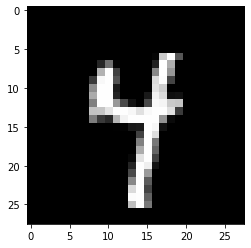
\includegraphics[width=0.25\columnwidth]{assets/output1.png}
  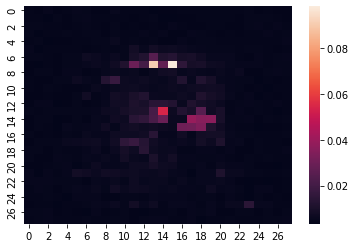
\includegraphics[width=0.5\columnwidth]{assets/output.png}
  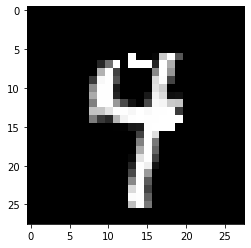
\includegraphics[width=0.25\columnwidth]{assets/output2.png}\\
  Original 5 Now 9\\
  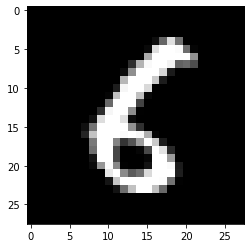
\includegraphics[width=0.25\columnwidth]{assets/output4.png}
  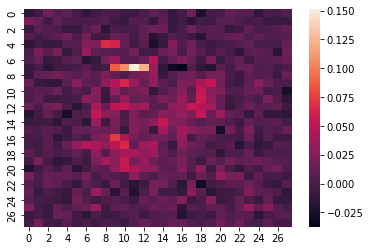
\includegraphics[width=0.5\columnwidth]{assets/output3.png}
  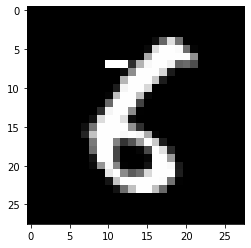
\includegraphics[width=0.25\columnwidth]{assets/output5.png}\\
  Original 6 Now 8
\item
  Train distillation model

  Based on the paper
  \href{https://arxiv.org/abs/1511.04508}{Distillation as a Defense to
  Adversarial Perturbations against Deep Neural Networks}\\
  I first processed the y\_train predicted by original model (10*1 array
  such as [0.1, 0.2, 0.3, 0.4, 0.5, 0.6, 0.7, 0.8, 0.9, 0.1]), then use it as y to train the new model

\begin{verbatim}
  Model: "sequential_38"
  _________________________________________________________________
   Layer (type)                Output Shape              Param #   
  =================================================================
   conv2d_61 (Conv2D)          (None, 26, 26, 32)        320       

   max_pooling2d_70 (MaxPoolin  (None, 13, 13, 32)       0         
   g2D)                                                            

   conv2d_62 (Conv2D)          (None, 11, 11, 64)        18496     

   max_pooling2d_71 (MaxPoolin  (None, 5, 5, 64)         0         
   g2D)                                                            

   flatten_41 (Flatten)        (None, 1600)              0         

   dropout_36 (Dropout)        (None, 1600)              0         

   dense_39 (Dense)            (None, 10)                16010     

  =================================================================
  Total params: 34,826
  Trainable params: 34,826
  Non-trainable params: 0
\end{verbatim}

\item
  Attack the distillation model

  Recall the multiply\_factor that controls the points added to the
  attacked image, this number reflects how \texttt{hard} to attack the
  model. As we have trained the distillation model, we want to validate
  that whether te proposed distillation model is more robust against
  attacks, so we randomly check what is the multiply\_factor to change
  the prediction of original model and distillation model, compare the
  multiply\_factor we can see the robustness of these 2 models.\\
  For example, the original image and the heatmap for attack points
  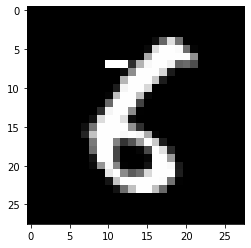
\includegraphics[width=0.25\columnwidth]{assets/output5.png} 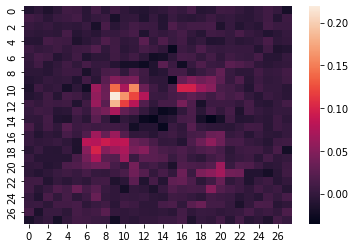
\includegraphics[width=0.5\columnwidth]{assets/output7.png}

  The minimum multiply\_factor to attack the original model is shown on
  left, and the minimum multiply\_factor to attack the distillation
  model is shown on the right side\\
  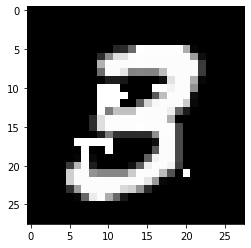
\includegraphics[width=0.25\columnwidth]{assets/output8.png}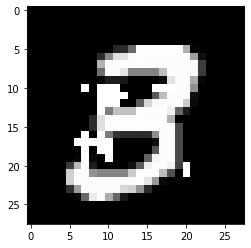
\includegraphics[width=0.25\columnwidth]{assets/output9.png}

  We can see it need few more points to attack the distillation model

  Then, we run tests on these 2 models and check the average
  multiply\_factor for original model and distillation model.

  And check 600 random images out of the train images, that the average
  factor to mislead the original model is 23, while the average for
  distillation model is 27, which shows the distillation model has
  better robustness than the original model
\end{enumerate}

References: {[}1{]} Papernot, Nicolas, et al.~``Distillation as a
defense to adversarial perturbations against deep neural networks.''
2016 IEEE symposium on security and privacy (SP). IEEE, 2016.\\
{[}2{]} Athalye, Anish, Nicholas Carlini, and David Wagner. ``Obfuscated
gradients give a false sense of security: Circumventing defenses to
adversarial examples.'' International conference on machine learning.
PMLR, 2018.\\
{[}3{]} MNIST Adversarial Examples Challenge
https://github.com/MadryLab/mnist\_challenge\\
{[}4{]} mnist-adversary https://github.com/dguliani/mnist-adversary\\
{[}5{]} Simple MNIST convnet
https://keras.io/examples/vision/mnist\_convnet/\\
{[}6{]} Help from friend Sida Zhu

\end{document}
